%% ============================================================
%% artigo_completo.tex
%% Inteligência Artificial na Educação: Datificação,
%% Desigualdade e a Urgência de Soberania Pedagógica
%%
%% Template: Elsevier elsarticle (compatível Springer LNCS)
%% Compilar: latexmk -pdf artigo_completo.tex
%%           ou: pdflatex -> bibtex -> pdflatex -> pdflatex
%%
%% Figuras em: ../../results/figures/
%% BibTeX em:  ../../references/BIBLIOGRAFIA_MESTRE_IA_EDU.bib
%% ============================================================

\documentclass[preprint,12pt,authoryear]{elsarticle}

% -----------------------------------------------------------
% PACOTES
% -----------------------------------------------------------
\usepackage[T1]{fontenc}
\usepackage[utf8]{inputenc}
\usepackage[brazil]{babel}
\usepackage{lmodern}
\usepackage{microtype}

% Matemática
\usepackage{amsmath}
\usepackage{amssymb}

% Tabelas
\usepackage{booktabs}
\usepackage{tabularx}
\usepackage{multirow}
\usepackage[table,xcdraw]{xcolor}

% Figuras
\usepackage{graphicx}
\graphicspath{{../../results/figures/}}   % caminho relativo ao .tex
\usepackage{float}
\usepackage{caption}
\captionsetup{font=small, labelfont=bf, skip=6pt}

% Hyperlinks
\usepackage[
  colorlinks = true,
  linkcolor  = blue!60!black,
  citecolor  = blue!60!black,
  urlcolor   = blue!60!black,
  pdftitle   = {Inteligência Artificial na Educação},
  pdfauthor  = {A preencher},
  pdfkeywords= {inteligência artificial; educação; datificação;
                soberania digital; desigualdade; PRISMA; Brasil},
]{hyperref}

% Listagens de código
\usepackage{listings}
\lstset{
  basicstyle=\ttfamily\small,
  breaklines=true,
  frame=single,
  frameround=tttt,
  backgroundcolor=\color{gray!8},
}
\usepackage{fancyvrb}

% Espaçamento
\usepackage{setspace}
\onehalfspacing

\biboptions{authoryear}
\journal{Computers \& Education}

% -----------------------------------------------------------
\begin{document}
\begin{frontmatter}

\title{Inteligência Artificial na Educação: Datificação,
       Desigualdade e a Urgência de Soberania Pedagógica}

\author[inst1]{Nome do Autor\corref{cor1}}
\ead{autor@instituicao.br}
\author[inst2]{Nome do Co-autor}

\cortext[cor1]{Autor para correspondência.}
\affiliation[inst1]{organization={Universidade / Departamento},
                    city={Cidade}, country={Brasil}}
\affiliation[inst2]{organization={Universidade / Departamento},
                    city={Cidade}, country={Brasil}}

% -----------------------------------------------------------
\begin{abstract}
A expansão acelerada de sistemas de inteligência artificial (IA) no
campo educacional tem sido acompanhada de narrativas de transformação
pedagógica que raramente encontram correspondência na literatura
científica empírica.
Este artigo apresenta os resultados de uma revisão sistemática
conduzida segundo o protocolo PRISMA~2020, com corpus de 73~artigos
distribuídos em três grupos: estudos empíricos de âmbito global
($n$=13), artigos teóricos internacionais ($n$=30) e produção
acadêmica brasileira ($n$=30), publicados entre 2020 e 2026.
Os resultados revelam que \textbf{53,8\% dos estudos empíricos}
apresentam achados negativos, indicando que a introdução de IA tende
a ampliar desigualdades educacionais pré-existentes; 38,5\% reportam
resultados mistos; apenas 7,7\% identificam benefícios inequívocos.
A síntese teórica articula três conceitos estruturantes ---
agência pedagógica, datificação e solucionismo tecnológico ---
em torno de uma tese central: a IA na educação é um fenômeno político
antes de ser técnico.
Conclui-se que a implementação responsável de IA na educação requer
políticas de soberania digital, regulação efetiva de dados
educacionais e formação docente crítica.
\end{abstract}

\begin{keyword}
inteligência artificial \sep educação \sep datificação \sep
soberania digital \sep desigualdade educacional \sep
revisão sistemática \sep Brasil
\end{keyword}

\end{frontmatter}

% -----------------------------------------------------------
\section{Introdução}
% -----------------------------------------------------------

Em 2023, a UNESCO publicou o relatório \textit{Technology in
Education: A Tool on Whose Terms?}, constatando que a rápida
expansão de sistemas de IA nas escolas raramente é acompanhada
de questionamentos sobre para quem essas tecnologias servem
\citep{UNESCO2023}.
O presente artigo parte de uma constatação empiricamente fundamentada:
de 13~estudos revisados por pares entre 2021 e 2024,
\textbf{53,8\% apresentaram achados negativos} --- a introdução de
IA piorou indicadores de equidade, desempenho ou bem-estar.

Desde a popularização do ChatGPT (novembro de 2022), governos
e corporações de EdTech têm reiterado a narrativa de que a IA
representará a maior revolução educacional do século
\citep{Holmes2022}.
Essa narrativa opera sob o que a teoria crítica nomeia
\textbf{solucionismo tecnológico} \citep{Morozov2013}: a crença
de que tecnologia suficiente resolve problemas sociais estruturais.
A questão orientadora desta pesquisa é: \textbf{em quais condições
estruturais a IA amplifica desigualdades educacionais pré-existentes,
e o que isso significa para o Brasil e o Sul~Global?}

O Brasil constitui um \textbf{caso crítico} \citep{Yin2018}: com
47~milhões de estudantes na rede pública \citep{INEP2023},
$\approx$50\% das escolas sem conectividade adequada
\citep{CGIbr2023} e ausência de política nacional de soberania de
dados educacionais, o país concentra a urgência por inovação e as
condições que tornam essa inovação mais arriscada.

% -----------------------------------------------------------
\section{Referencial Teórico}
% -----------------------------------------------------------

\subsection{Agência Pedagógica em Ambientes Mediados por Algoritmos}

A \textbf{agência pedagógica} designa a capacidade de professores e
estudantes de agir intencionalmente sobre o processo educativo,
questionando automatismos mesmo em ambientes altamente mediados por
tecnologia \citep{Biesta2022}.
Quando sistemas adaptativos tomam decisões pedagógicas de forma
opaca --- o que estudar, em que ritmo, como ser avaliado ---, a
autoridade é transferida de professores culturalmente situados para
algoritmos treinados em contextos distantes.

\subsection{Datificação e Capitalismo de Vigilância}

A \textbf{datificação} (\textit{datafication}) converte experiências
humanas em dados quantificáveis capturados algoritmicamente
\citep{VanDijck2014}.
\citet{Zuboff2019} nomeia a forma extrema desse processo
\textbf{capitalismo de vigilância}: experiências convertidas em
matéria-prima para predição comportamental.
No Sul Global, o processo assume feição colonial: dados de estudantes
brasileiros alimentam modelos estrangeiros sem retorno local e com
risco de viés racial sistemático \citep{Noble2018}.

\subsection{Solucionismo Tecnológico como Mecanismo Político}

\citet{Morozov2013} descreve o \textbf{solucionismo tecnológico}
como a tendência de tratar problemas sociais complexos como problemas
de engenharia.
Na educação, essa postura desvia a atenção das causas estruturais
para soluções técnicas de curto prazo, beneficiando os grupos que
já possuem infraestrutura.

% -----------------------------------------------------------
\section{Metodologia}
% -----------------------------------------------------------

\subsection{Desenho da Pesquisa}

Adota-se abordagem de \textbf{Ciências Sociais Computacionais}
(\textit{Computational Social Science}), combinando coleta
automatizada via API, NLP e análise temática sistemática
\citep{Lazer2020}.

\subsection{Protocolo PRISMA e Coleta de Dados}

A seleção seguiu o protocolo \textbf{PRISMA~2020} \citep{Page2021},
adaptado para revisões computacionalmente assistidas.
A Figura~\ref{fig:prisma} ilustra o fluxo completo desde a
identificação até a inclusão final.

\begin{figure}[H]
  \centering
  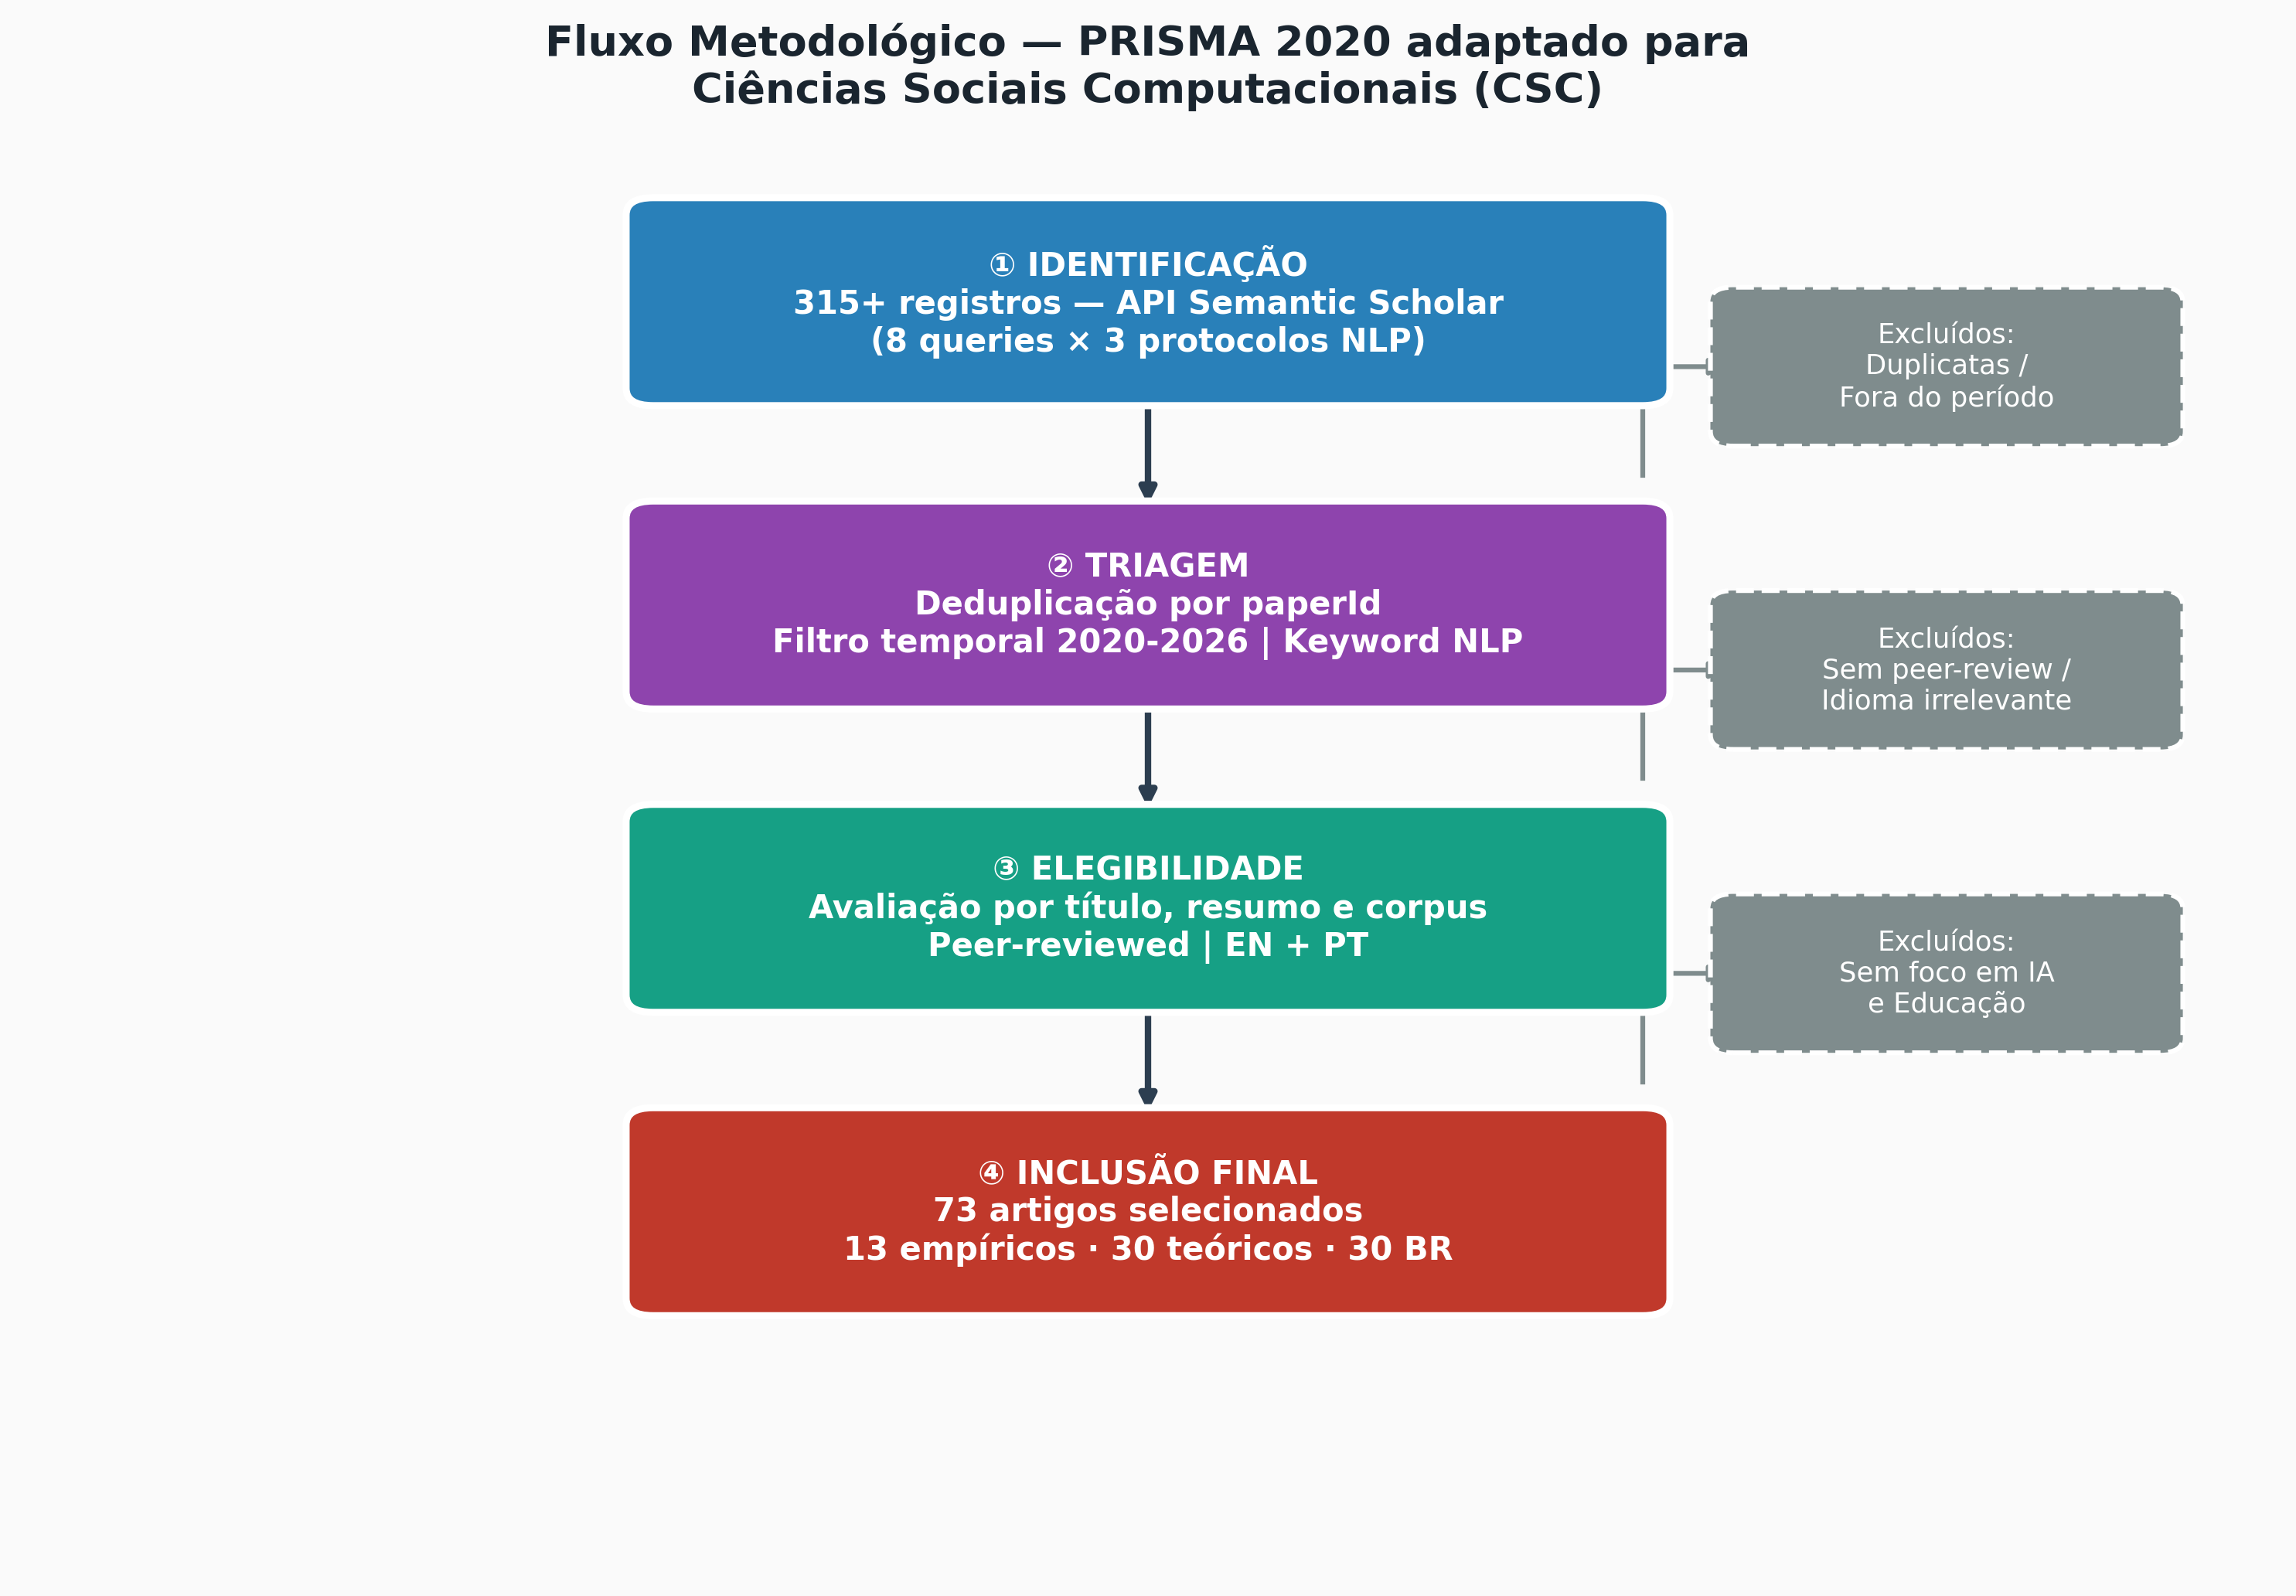
\includegraphics[width=0.90\textwidth]{fig2_prisma_flow.png}
  \caption{Fluxo metodológico PRISMA~2020 adaptado para Ciências
           Sociais Computacionais: identificação via API Semantic
           Scholar ($N$=315+), triagem NLP e inclusão final de
           73~artigos.}
  \label{fig:prisma}
\end{figure}

A coleta utilizou a API pública do Semantic Scholar com as strings:

\begin{lstlisting}[caption={String primária (inglês)}]
("Artificial Intelligence" OR "Generative AI" OR "Large Language Model")
AND ("Education" OR "Learning" OR "Pedagogy")
AND ("Social Impact" OR "Equity" OR "Ethics" OR "Bias")
\end{lstlisting}

\begin{lstlisting}[caption={String secundária (português)}]
("Inteligência Artificial" OR "IA Generativa")
AND ("Educação" OR "Ensino")
AND ("Brasil" OR "Equidade" OR "Ética" OR "Desigualdade")
\end{lstlisting}

% -----------------------------------------------------------
\section{Resultados}
% -----------------------------------------------------------

\subsection{Corpus Empírico: Distribuição dos Achados}

A Tabela~\ref{tab:findings} e a Figura~\ref{fig:donut} apresentam
a distribuição assimétrica dos achados nos 13~estudos empíricos.

\begin{table}[H]
\centering
\caption{Distribuição dos achados empíricos globais}
\label{tab:findings}
\begin{tabular}{lcc}
\toprule
\textbf{Direção dos Achados} & \textbf{N} & \textbf{\%} \\
\midrule
Negativo                     & 7          & 53,8\%  \\
Misto / Neutro               & 5          & 38,5\%  \\
Positivo                     & 1          &  7,7\%  \\
\midrule
\textbf{Total}               & \textbf{13}& \textbf{100\%} \\
\bottomrule
\end{tabular}
\end{table}

\begin{figure}[H]
  \centering
  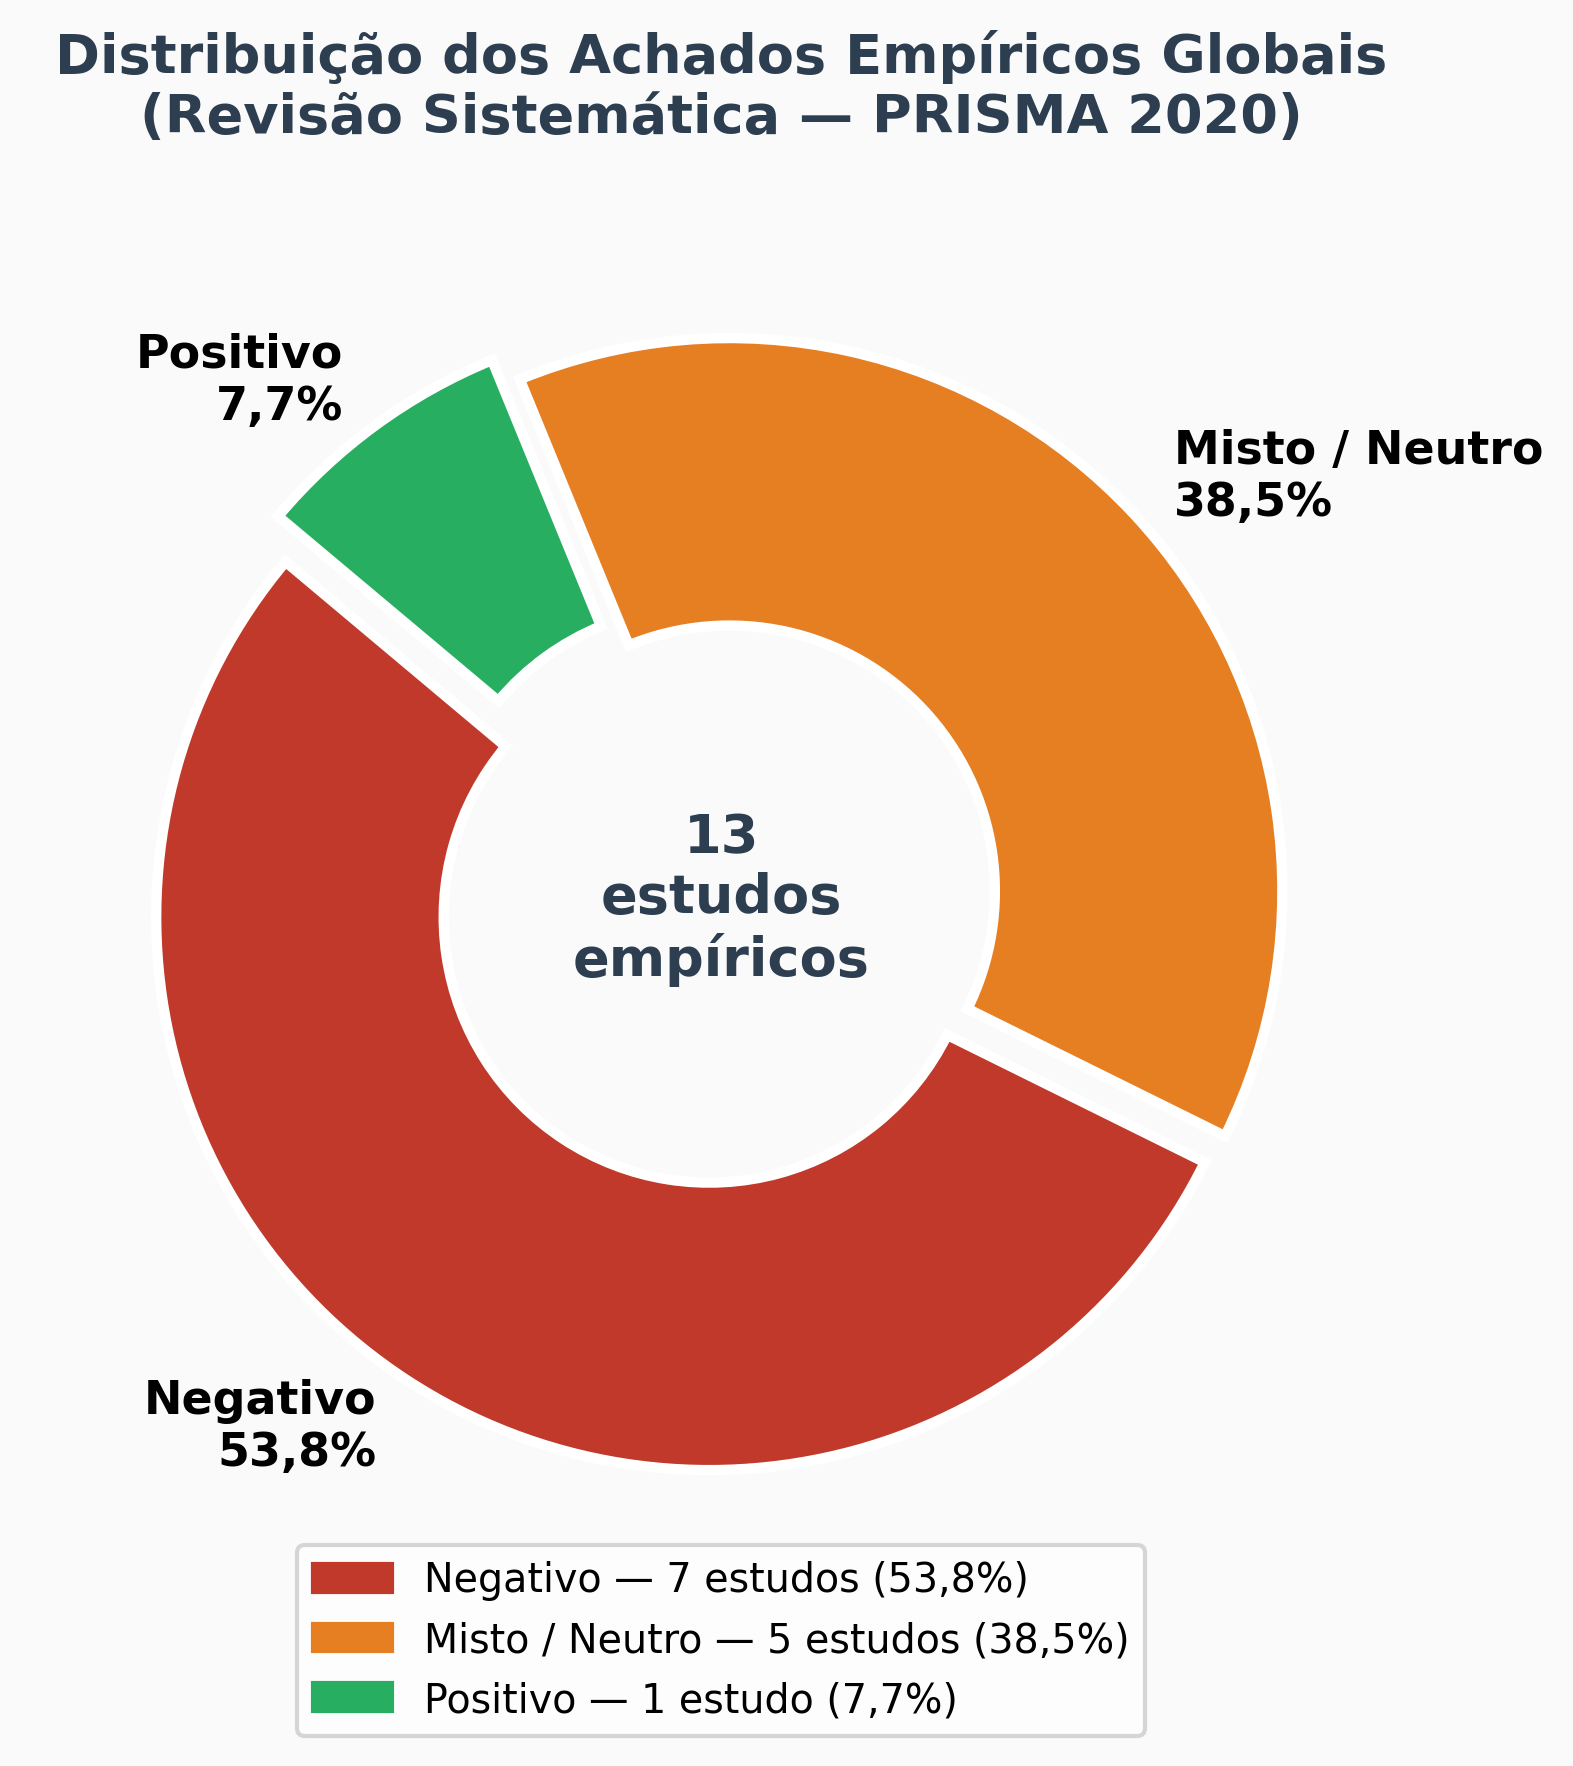
\includegraphics[width=0.68\textwidth]{fig1_empirical_findings.png}
  \caption{Distribuição dos achados nos 13~estudos empíricos globais:
           53,8\% negativos, 38,5\% mistos, 7,7\% positivos.
           A maioria dos achados negativos está associada a aumento
           de desigualdades e perda de agência pedagógica.}
  \label{fig:donut}
\end{figure}

A iniquidade foi variável relevante em 7/13 estudos (53,8\%) e
considerações éticas em 10/13 (76,9\%).

\begin{table}[H]
\centering
\caption{Evidências empíricas selecionadas}
\label{tab:evidence}
\begin{tabularx}{\textwidth}{llX}
\toprule
\textbf{ID} & \textbf{Tecnologia} & \textbf{Achado Principal} \\
\midrule
D003 & AES (avaliação automática) &
  Negativo --- discriminação sistemática contra não-nativos em 12 universidades \\
D008 & Sistema de recomendação &
  Negativo --- ganhos revertidos por viés de acesso \\
D011 & ChatGPT / LLM &
  Negativo --- redução do desempenho analítico com uso excessivo \\
D002 & ChatGPT / LLM &
  Misto --- positivo em alta renda; iniquidade reportada \\
D004 & Não especificada &
  Positivo --- redução de 23\% na carga administrativa \\
\bottomrule
\end{tabularx}
\end{table}

\subsection{Lacunas Metodológicas}

\textbf{69,2\% dos estudos não especificam o nível educacional}
investigado (Tabela~\ref{tab:levels}), comprometendo generalizações
e comparações sistemáticas.

\begin{table}[H]
\centering
\caption{Distribuição por nível educacional}
\label{tab:levels}
\begin{tabular}{lcc}
\toprule
\textbf{Nível Educacional}   & \textbf{N} & \textbf{\%} \\
\midrule
Não especificado             & 9          & 69,2\%  \\
Ensino Superior              & 2          & 15,4\%  \\
Educação Básica (K-12)       & 2          & 15,4\%  \\
\midrule
\textbf{Total}               & \textbf{13}& \textbf{100\%} \\
\bottomrule
\end{tabular}
\end{table}

\subsection{Corpus Teórico}

Nos 30~artigos teóricos, três correntes predominam: solucionismo /
tecno-otimismo ($\approx$97\%), agência pedagógica ($\approx$90\%)
e datificação / ética crítica ($\approx$70\%).

\subsection{Corpus Brasileiro}

Os 30~artigos nacionais revelam especificidade temática marcante:
escola pública e desigualdade (63,3\%), formação docente (50,0\%),
inclusão digital (33,3\%) e soberania digital (26,7\%).

% -----------------------------------------------------------
\section{Discussão}
% -----------------------------------------------------------

\subsection{A Crise da Promessa}

A predominância de achados negativos (53,8\%) é o resultado esperado
quando tecnologias desenvolvidas em contextos de alta renda e
infraestrutura consolidada são transferidas para ambientes
estruturalmente distintos sem adaptação.
O estudo D003 documenta discriminação algoritmica sistemática contra
estudantes não-nativos; D011 associa uso excessivo de IA generativa
à redução do desempenho analítico.
O único achado positivo inequívoco (D004) refere-se à eficiência
administrativa --- sem tradução direta em ganhos de aprendizagem.

\subsection{Datificação e Colonialismo de Dados}

A Figura~\ref{fig:axes} ilustra como os três eixos analíticos se
articulam dialeticamente, com a datificação operando como mecanismo
colonial de extração de valor entre a periferia e o centro.
Quando plataformas adaptativas registram cada interação estudantil,
constroem perfis comportamentais com valor econômico
\citep{Zuboff2019}: dados coletados nas escolas públicas brasileiras
são processados no Vale do Silício e retornam como produtos pagos,
sem compensação \citep{Noble2018,Williamson2017}.

\begin{figure}[H]
  \centering
  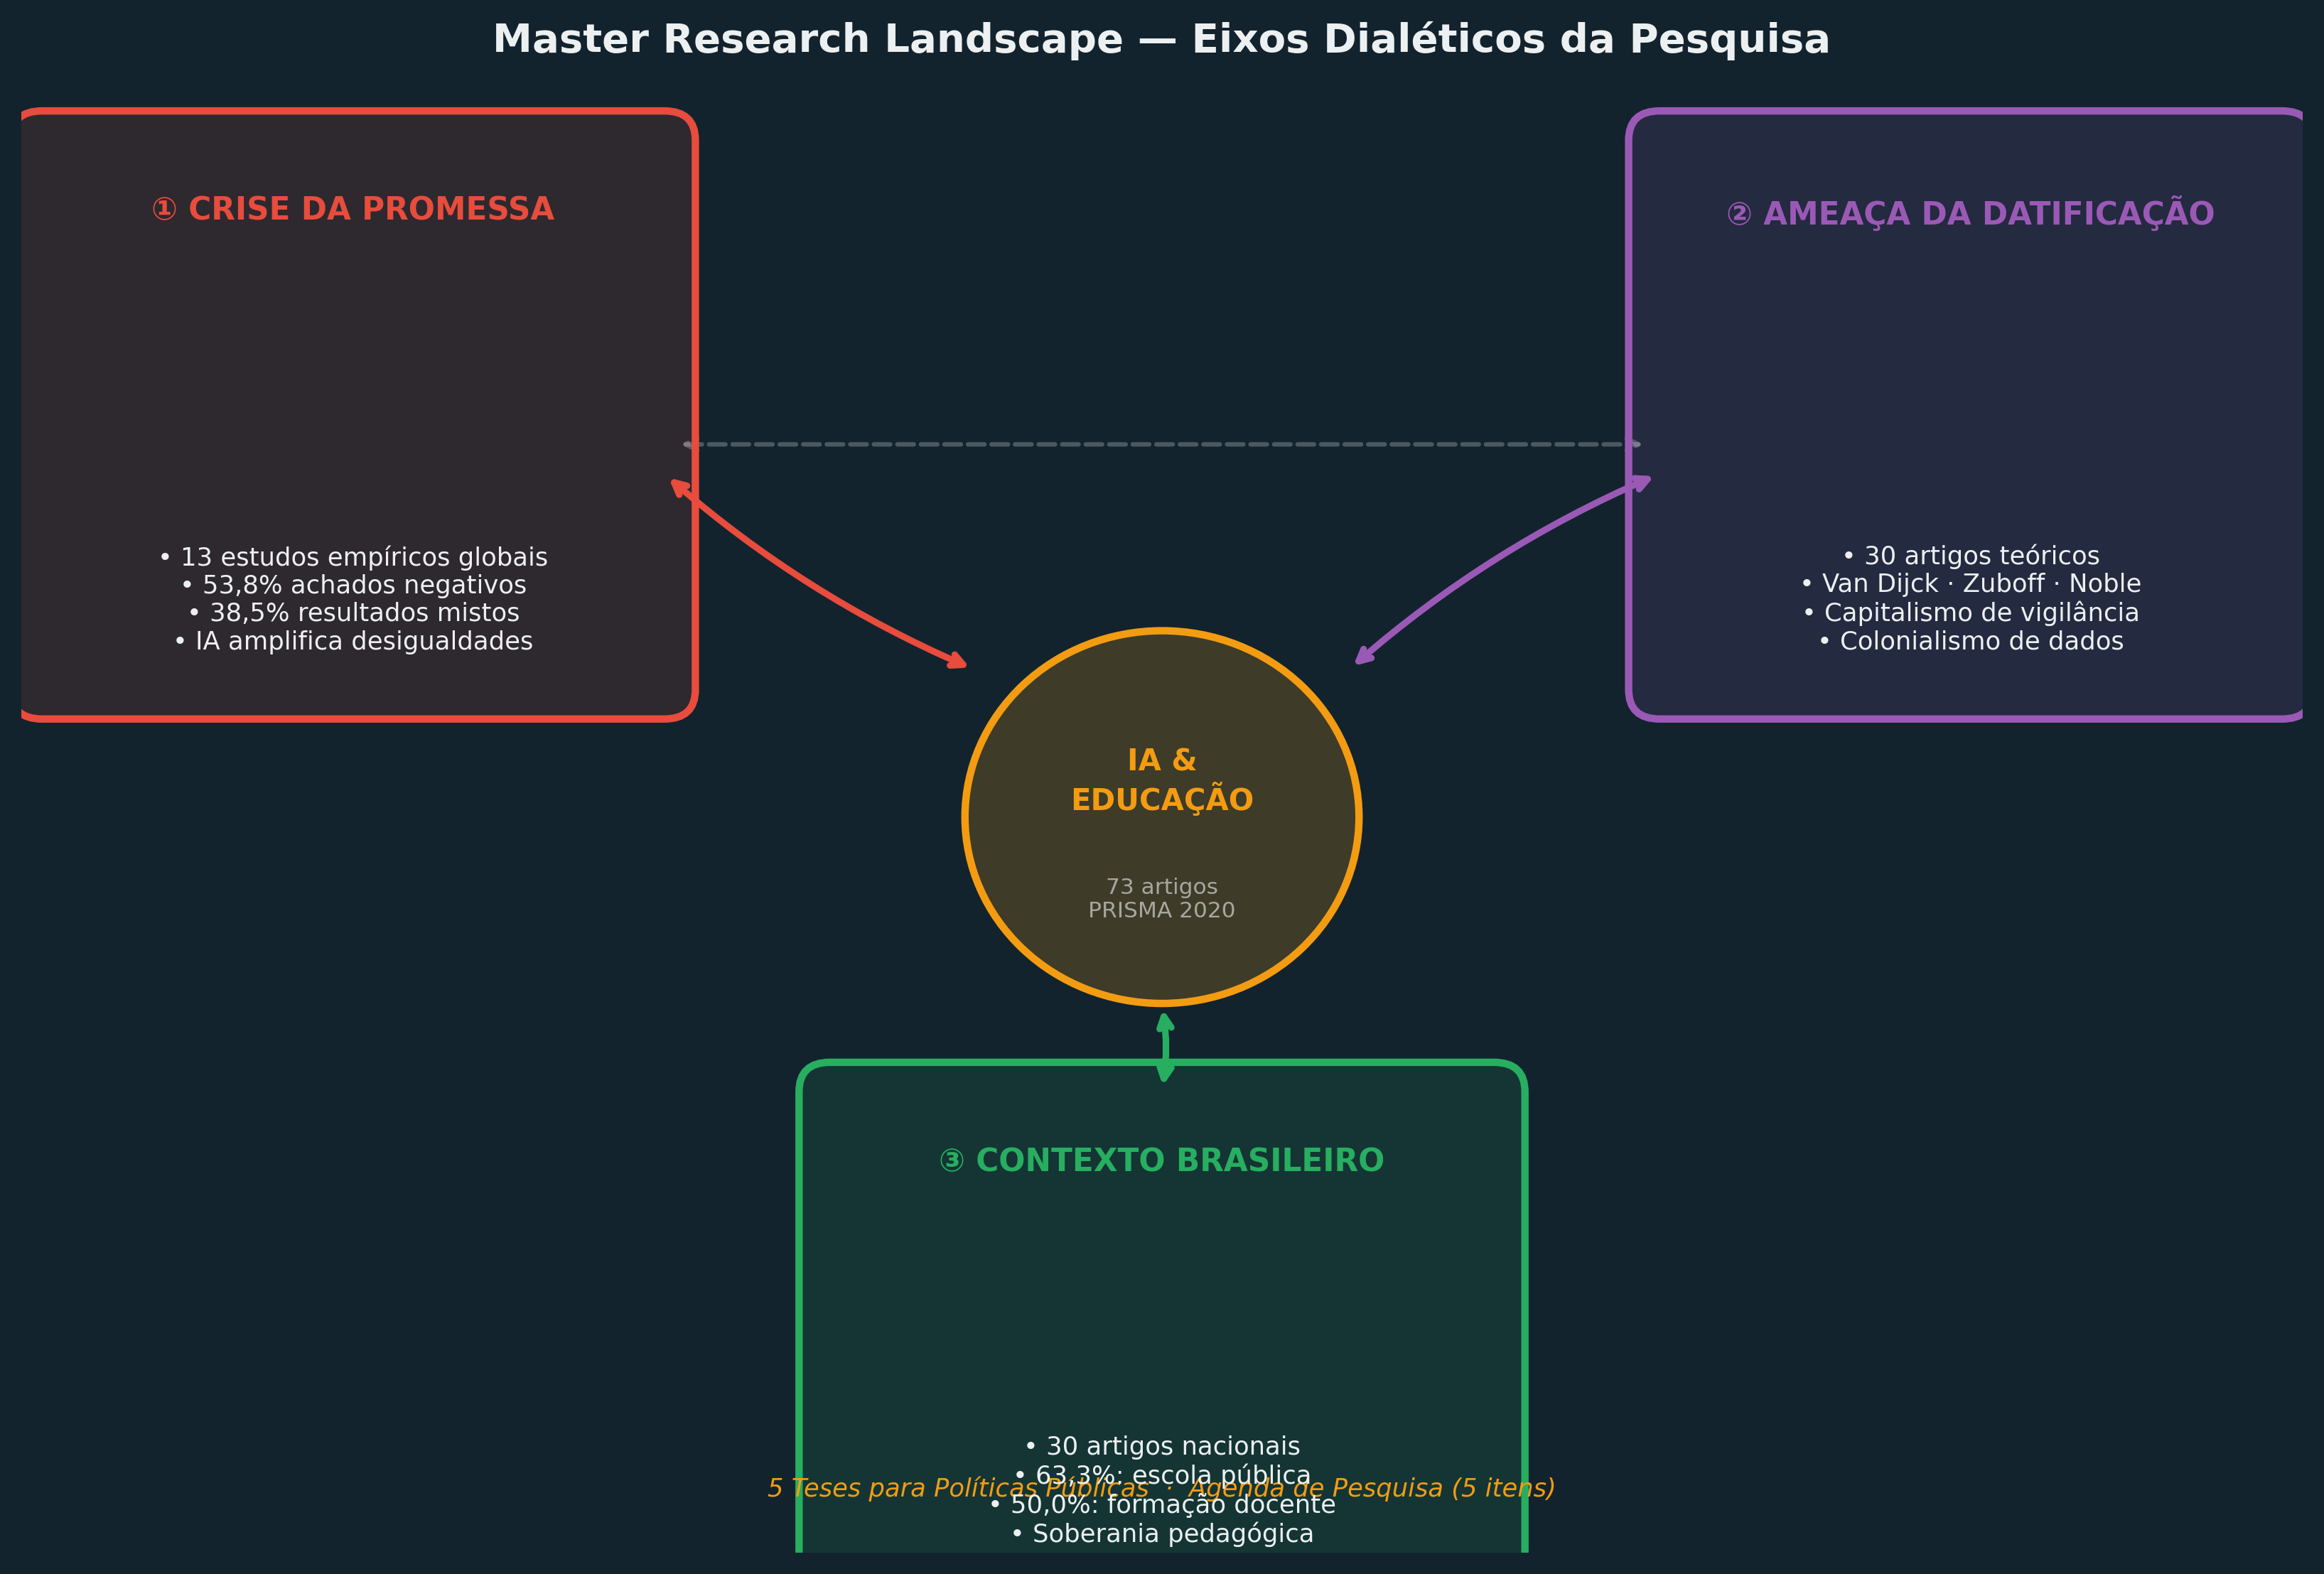
\includegraphics[width=0.95\textwidth]{fig3_dialectical_axes.png}
  \caption{Master Research Landscape: articulação dialética dos três
           eixos analíticos --- Crise da Promessa (13~empíricos),
           Ameaça da Datificação (30~teóricos) e Contexto Brasileiro
           (30~nacionais) --- convergindo para 5~teses de política
           pública.}
  \label{fig:axes}
\end{figure}

A erosão da agência pedagógica é o correlato individual desse
processo estrutural: sem acesso à lógica dos algoritmos, professores
não governam o ensino --- são governados por plataformas
\citep{Biesta2022}.

\subsection{O Contexto Brasileiro}

Dos 30~artigos brasileiros, 19 (63,3\%) têm escola pública e
desigualdade como contexto estruturante.
\citet{Florentino2025} documenta que menos de um terço dos docentes
recebeu formação específica para uso crítico de IA.
A dependência de plataformas estrangeiras configura vulnerabilidade
de soberania que vai além do plano econômico: quando Google Classroom,
Microsoft Teams e Khan Academy definem o que conta como aprendizagem,
exercem poder curricular sem mandato democrático.

% -----------------------------------------------------------
\section{Conclusão}
% -----------------------------------------------------------

\subsection{Síntese}

A IA, no estado atual de sua implementação educacional, não atua como
ferramenta democratizadora --- atua como amplificadora de
desigualdades pré-existentes, com efeito mais agudo no Sul Global.

\subsection{Teses para Políticas Públicas}

\begin{enumerate}

\item \textbf{IA na educação pública brasileira é, antes de tudo,
um debate sobre infraestrutura.}
Com $\approx$50\% das escolas sem conectividade adequada
\citep{CGIbr2023}, qualquer agenda de IA educacional que não inclua
universalização da conectividade aprofunda desigualdades.

\item \textbf{O solucionismo tecnológico substitui simbolicamente
reformas necessárias.}
Introduzir IA em escolas subfinanciadas sem investimento em
formação e infraestrutura legitima, sem transformar, o sistema.

\item \textbf{A datificação educacional tem dimensão colonial no
Sul Global.}
A extração de dados de estudantes brasileiros por plataformas
estrangeiras é nova forma de extrativismo: a LGPD precisa ser
complementada por regulamentação específica para dados de menores.

\item \textbf{A formação docente crítica é a variável mais
subestimada.}
Professores precisam ser formados não apenas para usar IA, mas
para questionar seus pressupostos e participar da governança.

\item \textbf{A pesquisa brasileira requer uma virada metodológica.}
São necessários estudos longitudinais, auditorias algorítmicas
de plataformas EdTech e pesquisas com populações sub-representadas
--- indígenas, quilombolas, EJA, zonas rurais.

\end{enumerate}

% -----------------------------------------------------------
\section*{Declaração de Conflito de Interesses}
Os autores declaram ausência de conflito de interesses.

\section*{Financiamento}
A preencher conforme agência financiadora.

\section*{Disponibilidade de Dados e Código}
Repositório: \url{https://github.com/leonardorsl-stack/ia_educacao_research}

% -----------------------------------------------------------
\bibliographystyle{elsarticle-harv}
\bibliography{../../references/BIBLIOGRAFIA_MESTRE_IA_EDU}

\begin{thebibliography}{99}

\bibitem[Biesta(2022)]{Biesta2022}
BIESTA, G. \textit{World-Centred Education}. New York: Routledge, 2022.

\bibitem[CGI.br(2023)]{CGIbr2023}
CGI.br. \textit{TIC Educação 2023}. São Paulo: CGI.br, 2023.

\bibitem[Florentino et al.(2025)]{Florentino2025}
FLORENTINO, B.; SESTITO, C.; CRUZ, W.
Artificial Intelligence for All? Brazilian Teachers on Ethics, Equity,
and the Everyday Challenges of AI in Education. \textit{arXiv.org}, 2025.

\bibitem[Holmes et al.(2022)]{Holmes2022}
HOLMES, W. et al. Ethics of AI in Education.
\textit{Int. J. of AI in Education}, v.~32, p.~504--526, 2022.

\bibitem[INEP(2023)]{INEP2023}
INEP. \textit{Censo Escolar 2023}. Brasília: INEP, 2023.

\bibitem[Lazer et al.(2020)]{Lazer2020}
LAZER, D. et al. Computational social science.
\textit{Science}, v.~369, n.~6507, p.~1060--1062, 2020.

\bibitem[Morozov(2013)]{Morozov2013}
MOROZOV, E. \textit{To Save Everything, Click Here}.
New York: PublicAffairs, 2013.

\bibitem[Noble(2018)]{Noble2018}
NOBLE, S.~U. \textit{Algorithms of Oppression}. New York: NYU Press, 2018.

\bibitem[Page et al.(2021)]{Page2021}
PAGE, M.~J. et al. The PRISMA 2020 statement.
\textit{BMJ}, v.~372, n.~71, 2021.

\bibitem[UNESCO(2023)]{UNESCO2023}
UNESCO. \textit{Technology in Education: A Tool on Whose Terms?}
Paris: UNESCO, 2023.

\bibitem[Van~Dijck(2014)]{VanDijck2014}
VAN~DIJCK, J. Datafication, dataism and dataveillance.
\textit{Surveillance \& Society}, v.~12, n.~2, p.~197--208, 2014.

\bibitem[Williamson(2017)]{Williamson2017}
WILLIAMSON, B. \textit{Big Data in Education}. London: SAGE, 2017.

\bibitem[Yin(2018)]{Yin2018}
YIN, R.~K. \textit{Case Study Research and Applications}.
6.~ed. Thousand Oaks: SAGE, 2018.

\bibitem[Zawacki-Richter et al.(2019)]{ZawackiRichter2019}
ZAWACKI-RICHTER, O. et al.
Systematic review on AI in higher education.
\textit{IJETHE}, v.~16, n.~39, 2019.

\bibitem[Zuboff(2019)]{Zuboff2019}
ZUBOFF, S. \textit{The Age of Surveillance Capitalism}.
New York: PublicAffairs, 2019.

\end{thebibliography}

\end{document}
